% file: main.tex
%\documentclass{report}ss[12pt,oneside]{book}
%\usepackage[final]{feynmf}
\documentclass[12pt]{report}
\usepackage[centertags]{amsmath}
\usepackage{amsfonts}
\usepackage{amssymb}
\usepackage{amsthm}
\usepackage{graphicx}
\usepackage{newlfont}
\usepackage{fancyhdr}
\usepackage{appendix}
\usepackage{hyperref}
\usepackage{makeidx}
\usepackage{waqar} % COMSATS adjusted for Style
\usepackage{XTocinc} %Include Table of Contents as the first entry in TOC
\usepackage{nomencl}
\usepackage{url}
\usepackage[english]{babel}
\usepackage{multirow}
%\makenomenclature
%                     Faculty of Grad Studies insists on this!?
%\usepackage[active]{srcltx}  %SRC Specials for DVI search
% Fuzz -------------------------------------------------------------------
\hfuzz2pt % Don't bother to report over-full boxes if over-edge is < 2pt
% Line spacing -----------------------------------------------------------
\newlength{\defbaselineskip}
\setlength{\defbaselineskip}{\baselineskip}
\newcommand{\setlinespacing}[1]%
           {\setlength{\baselineskip}{#1 \defbaselineskip}}
\newcommand{\doublespacing}{\setlength{\baselineskip}%
                           {2.0 \defbaselineskip}}
\newcommand{\singlespacing}{\setlength{\baselineskip}{\defbaselineskip}}
% MATH -------------------------------------------------------------------
\newcommand{\A}{{\cal A}}
\newcommand{\h}{{\cal H}}
\newcommand{\s}{{\cal S}}
\newcommand{\W}{{\cal W}}
\newcommand{\BH}{\mathbf B(\cal H)}
\newcommand{\KH}{\cal  K(\cal H)}
\newcommand{\Real}{\mathbb R}
\newcommand{\Complex}{\mathbb C}
\newcommand{\Field}{\mathbb F}
\newcommand{\RPlus}{[0,\infty)}
%
\newcommand{\norm}[1]{\left\Vert#1\right\Vert}
\newcommand{\essnorm}[1]{\norm{#1}_{\text{\rm\normalshape ess}}}
\newcommand{\abs}[1]{\left\vert#1\right\vert}
\newcommand{\set}[1]{\left\{#1\right\}}
\newcommand{\seq}[1]{\left<#1\right>}
\newcommand{\eps}{\varepsilon}
\newcommand{\To}{\longrightarrow}
\newcommand{\RE}{\operatorname{Re}}
\newcommand{\IM}{\operatorname{Im}}
\newcommand{\Poly}{{\cal{P}}(E)}
\newcommand{\EssD}{{\cal{D}}}

% THEOREMS ---------------------------------------------------------------
\theoremstyle{plain}
\newtheorem{thm}{Theorem}[section]
\newtheorem{cor}[thm]{Corollary}
\newtheorem{lem}[thm]{Lemma}
\newtheorem{prop}[thm]{Proposition}
%
\theoremstyle{definition}
\newtheorem{defn}{Definition}[section]
%
\theoremstyle{remark}
\newtheorem{rem}{Remark}[section]
%
\numberwithin{equation}{section}
\renewcommand{\theequation}{\thesection.\arabic{equation}}
% ----------------------------------------------------------------------
\setlength{\tclineskip}{1.25\baselineskip}
% ----------------------------------------------------------------------
%\nobib
%\draft
%\nofront

%\permissionfalse
\dedicate{To my family.}
\copyrightyear{\today}
\submitdate{\today}
%\convocation{July}{2016}

% ------------------------------------------------------------------------
\makeindex

\pagestyle{fancy}
\fancyhead[LE,RO]{\slshape\rightmark}
\fancyhead[LO,RE]{\slshape\leftmark}
\renewcommand{\headrulewidth}{0.4pt}
\renewcommand{\footrulewidth}{0 pt}
%\renewcommand{\chaptermark}[1]{ \markboth{\chaptername \thechapter.\ #1}{}}

%\renewcommand{\sectionmark}[1]{\markboth{\MakeUppercase {\thesection.\ #1}}{}}
%\renewcommand{\sectionmark}[1]{\markright{\thesection.\ #1}}

% ------------------------------------------------------------------------

\begin{document}
\title{Tripple GEM Trigger and DAQ system using $\mu$TCA at CMS upgrade. }
\author{Waqar Ahmed}
\supervisor{\textbf {Prof.Dr.Shahid A. Khan}\\Dean-HOD \\Department of Electrical Engineering.
\\COMSATS Institute of Information Technology    \\Islamabad,Pakistan}
\degree{Philosophy of Doctoral} \degreeinitial{Ph.D}
%\Supervisor{\textbf {Prof.Dr. Gilles De Lentdecker} \\Head
%\\Data Acquisation System CMS CERN\\Geneva, Switzerland\\ Professor University of Brusel Baljium}
\beforepreface 
%------------------------------------------------------------------------
% ************************** Thesis Abstract *****************************
% Use `abstract' as an option in the document class to print only the titlepage and the abstract.
\begin{abstract}
The developments were rather generic, driven by the observation that modern technologies allow to design a DAQ architecture independent of the detector technology to which the DAQ system will be connected, providing freedom to the choice of the future experiment. It becomes clear now that the future particle and astro-particle experiments plan to use the most advanced technologies from the telecommunication and the digital programmable electronic industries: the Advanced Telecom Computing Architecture (ATCA or micro-TCA) standard and Field Programmable Gate Arrays (FPGA).Currently we are working on design of the DAQ system of the CMS Forward Muon Upgrade project which proposes to install Triple-GEM detectors instead of Resistive Plate Chambers in the first CMS muon station at 1.6 <$\eta$< 2.4 during the 2nd LHC long shutdown. The IIHE is also leading the design of the DAQ system of Askaryan Radiotelescope Array (ARA) project, for which radio-antennas are being spread over an area of several km2 in the South Pole ice, close to the IceCube experiment. In addition the IIHE contributes to the DAQ development of the Large TPC prototype for the ILC. In the framework of the CMS upgrades, the IIHE in collaboration with the University of Antwerpen is investigating the new micro-TCA standard, introduced by the telecommunication industry, to replace the VME electronics. With its high data throughput (several Gbps), high reliability and high availability, the micro-TCA standard combined with the most powerful FPGAs for the data processing should allow the future CMS DAQ system to cope with the LHC luminosity beyond the nominal value of 10$^{33}$ cm$^{-2}$s$^{-1}$.
Typically these systems require high data volume transmission, from 0.5 to 3.2 Gbps, from the detector to off-detector electronics where data are processed by FPGAs, as well as the distribution of precise signals like clock and trigger inputs towards the detectors. The high bandwidth transmission uses optical fibre transceivers and gigabit transceiver blocks (GTPs) routinely built into FPGA devices. We have also set-up a micro-TCA test bench equipped with various Advance Mezzanine Cards (AMC), either commercial ones or designed by IIHE electronic engineers. In particular we are evaluating the CERN’s Gigabit Link interface Board (GLIB) designed to test the GBT/Versatile optical link being developed by CERN for the next Tracker upgrade.

The micro-TCA technology is a relatively new telecommunication standard. It is planned to replace VME as the default technology for future particle physics experiments (LHC upgrades, ILC experiments, etc.). Consequently it still needs a lot of developments and specification validation for particle physics. Another aspect we are starting to develop is the implementation of complex algorithms on FPGAs. Indeed with the introduction of increasingly powerful FPGAs, it seems now feasible to run on such devices more advanced algorithms for trigger and track reconstruction.  These developments are of interest for the LHC trigger upgrades and in particular for the future CMS track trigger.
 
\end{abstract}

%------------------------------------------------------------------------
% ------------------------------------------------------------------------
% -*-TeX-*- -*-Hard-*- Smart Wrapping
% ------------------------------------------------------------------------
% Thesis Acknowledgements ------------------------------------------------

\prefacesection{Acknowledgements}
\def\baselinestretch{0.5}
\setlinespacing{1.25}

I would like to thank Prof.Dr.Shahid A Khan my supervisor,
and Prof.Dr.Gilles Landeckar my Co-Supervisor for
many suggestions and constant support during this
research. He shared his knowledge and provided many useful
references and friendly encouragements. I am thankful to my colleagues
their positive criticism, continuous support and courage
through the early stages of chaos and confusion.\\

\indent\smallskip I am grateful to the Director Genral (NCP) Prof. Dr. Hafeez Hoorani, for allowing me to do research in National Center for Physics and Provide me fund to reaserch at European Council for Nuclear Research (CERN) to complete major part of this thesis.\\


\noindent
\begin{flushright}
Waqar Ahmed\\
\end{flushright}

% ----------------------------------------------------------------------


% ------------------------------------------------------------------------
\afterpreface %\pagestyle{headings} 

\pagestyle{fancy}
\fancyhead[LE,RO]{%\slshape 
		\rightmark}
\fancyhead[LO,RE]{%\slshape 
		 \leftmark}
\renewcommand{\headrulewidth}{0.4pt}
\renewcommand{\footrulewidth}{0 pt}
\renewcommand{\sectionmark}[1]{\markboth{\MakeUppercase {\thesection.\ #1}}{}}
%\renewcommand{\sectionmark}[1]{\markright{\thesection.\ #1}}

% ------------------------------------------------------------------------
\setlinespacing{1.1}
% ------------------------------------------------------------------------
% ------------------------------------------------------------------------
% -*-TeX-*- -*-Hard-*- Smart Wrapping
% ------------------------------------------------------------------------
% Thesis Acknowledgements ------------------------------------------------

\prefacesection{My Contribution}
\def\baselinestretch{0.5}
\setlinespacing{1.25}


One of the characteristics of the experiments in the field of the High Energy
Physics is that they are based on the teamwork. In the CMS experiment a few thousands of
scientists, engineers and technicians were involved. Hence, it is obvious that not all issues
discussed in this thesis are my exclusive contribution.
The GEM detector trigger and DAQ sytem was proposed and designed by the Université libre de Bruxelles CMS
group, the group developed most of the custom electronic boards of the trigger system,
prepared the firmware for the FPGA devices, carried out the production and installation of the
trigger electronics. The GEM chambers were developed and produced by the scientists from
Italy, USA, Pakistan, Beljium, India and CERN. The Brussel CMS group have consisted
of a few dozens of people from the de de l'Université libre de Bruxelles. I have been a member of the group for over three years. My tasks included: software development, testing the prototypes of the electronic boards, testing the GEM detectors and DAQ system during installation, proposing the firmware improvements and modifications, work on the optohybird modules.
The on-line software for the PAC Trigger system, that is the subject of the
Chapter 4, was developed mainly by two people: Michał Pietrusiński and me. Michał was themain architect of the software structure and implemented most of the low-level software.
Based on that part, I have designed and implemented the test procedures for the trigger system
as well as details of the hardware configuration process. Additionally, my task was to decide
what diagnostic and monitoring tools should be implemented in the firmware of the trigger
electronics and how to analyse and present the data acquired by those tools. The dedicated
monitoring procedures were developed mostly by me and are a part of the PACT system
online software. 
The hardware and firmware solutions for the synchronization of the chamber data
and transmission channels were created by the main developer of the firmware for the PAC
system – Yifan young. My task was to find the ways of using those solutions in
practice. I have worked out the methods for finding the optimal values of the synchronization
parameters and implemented them in the dedicated software procedures, which allowed
successful synchronization of the VFAT signal to optohybrid module. (at the moment for the cosmic muons). The
analysis of the system synchronization from the data acquired during the cosmic muon runs,
as well as the simulation of the muon hits timing, was performed by other members of the
Brussel CMS group.

% ------------------------------------------------------------------------
% -*-TeX-*- -*-Hard-*- Smart Wrapping
% ------------------------------------------------------------------------
\def\baselinestretch{1}
%\pagestyle{headings}

\chapter{Compact Muon Solenoid Experiment and LHC }

%\def\baselinestretch{1.5}


%%% ----------------------------------------------------------------------
This chapter gives an introduction to the Large Hadron Collider
(LHC)~\cite{lhc} and Compact Muon Solenoid (CMS)~\cite{cms}
built by European Organization for Nuclear Research (CERN)
located at French-Swiss border near Geneva. There are four
experiments which will take place at LHC: two general purpose
detectors ATLAS~\cite{atlas} , CMS~\cite{cms}, and two
dedicated detectors LHC-b~\cite{lhcb} and ALICE~\cite{alice}
which will study b physics and heavy ion physics respectively.
The figure shows the four experimental sights along the LHC
ring. CMS is one of the major experiments being operated at LHC
near the village of Cessey France which will take data of both
p-p and Pb-Pb collisions.

\smallskip

%%% ----------------------------------------------------------------------
\goodbreak
\section{Large Hadron Collider}

LHC ring has just completed its installation at CERN and first
proton beam was injected in the beam pipe in September 2008.
LHC uses the former Large Electron Positron Collider (LEP)
tunnel with 27 km circumference. The main physics goal is the
    \begin{figure}[h]
    \begin{center}
    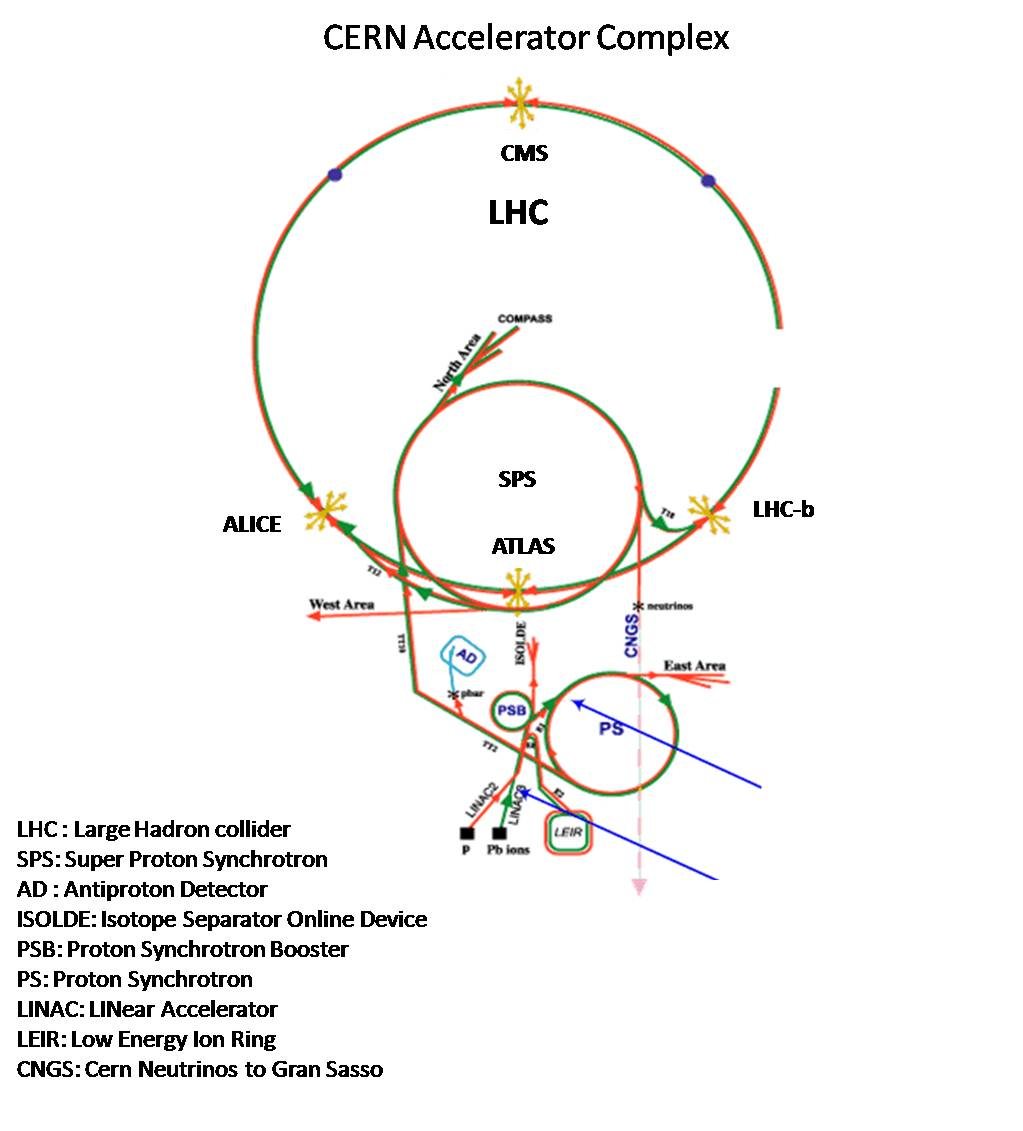
\includegraphics[width=3.5in, height= 4.0in]{pic/complex} \\
    \caption{CERN accelerator complex}
    \end{center}
    \end{figure}
search of Higgs boson and the testing of the standard Model of
particle physics at the energy scale of 1 TeV. The LHC will be
operated with proton-proton and heavy ion collisions with a
center of mass energy of 14 TeV for proton-proton collision and
5.5 TeV for heavy ion collisions with a luminosity of $10^{34}$
cm$^{-2}$s$^{-1}$ and $10^{28}$ cm$^{-2}$s$^{-1}$ respectively.
To achieve the design luminosity for p-p collision two beams
with 2800 bunches are injected into the beam pipe with 25 ns
gap. To keep the particles in track 1232 superconducting dipole
magnets producing a field of 8.3 Tesla are used. The figure 1.1
shows the schematic view of the CERN accelerator complex.

\bigskip
\section{Compact Muon Solenoid}

One of the general purpose detector CMS is located near the
village of Cessey France. The high luminosity and short bunch
spacing of LHC beam demanded a sophisticated detector. CMS
detector is a very compact as compared to the other general
purpose detector ATLAS which has more than twice the volume of
CMS. CMS detector has an excellent muon system assisted by
central tracking detector and solenoid produces a magnetic
field twice large as used by ATLAS. This allows the accurate
particle momentum measurement. The Figure~\ref{fig:1b} below
shows perspective view of the CMS detector.
    \begin{figure}[h]
    \begin{center}
    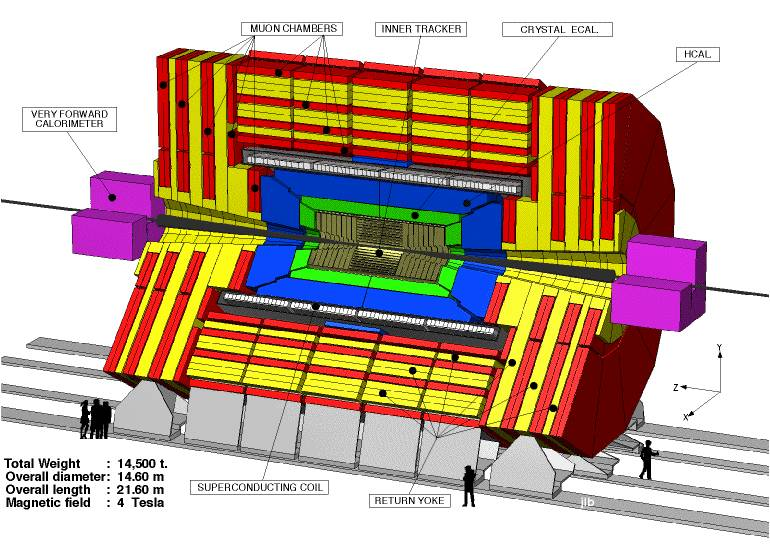
\includegraphics[width=3.5in]{pic/cms-pic} \\
    \caption{Longitudinal view of CMS Detector.}\label{fig:1b}
    \end{center}
    \end{figure}

The overall dimension of the CMS detector are 22 m in length 15
m in diameter with a total mass of 12500 tons. The coordinate
conventions are as follows: The interaction point which lies in
the middle of barrel part of the CMS where the two beams
collides is referred as the origin of the coordinate system.
The \emph{x}-axis points radially inward to the center of the
LHC ring. The \emph{z}-axis points along the direction of the
beam pipe and the \emph{y}-axis points vertically to the
surface. The azimuthal angle $\phi$ is measured in the
\emph{x-y}- plane from \emph{x}-axis. In the \emph{y-z}-plane
the angle $\theta$ is measured form \emph{z}-axis. The pseudo
rapidity is defined as $\eta=-\ln(\tan(\theta/2))$. A more
details of CMS experiment can be found
in~\cite{{cms-tdr1},{tdr2}}.

\smallskip

\subsection{Inner Tracking System}
Tracking system of CMS is designed to take the huge particle
flux coming for LHC collisions. The CMS tracker consists of
about 20000 silicon sensors with a total area of 210 m$^{2}$
having a diameter and length of about 2.4 m and 5.4 m
respectively thus its acceptance is up to $\eta<2.5$. Tracker
is located directly around the interaction point therefore it
receives a very high particle flux. Per bunch crossing around
1000 charged particles will hit the tracker at the radius of
about 4 cm therefore at such a distance the tracker has to be
radiation hard. The inner tracker mainly consist of silicon
pixel detector and silicon strip sensors. The whole system is
surrounded my 4 Tesla homogenous magnetic field~\cite{karim}.



\smallskip
\subsection{Silicon Pixel Tracker}
The pixel tracker is subdivided into two parts: First, three
cylindrical barrels located at radii of 4.4, 7.3 and 10.2 cm
around the interaction point with a length of 53 cm. Second, on
each side of the barrel two discs complement the tracker at
\emph{z} = $\pm32.5$ and $\pm$ 46.5 cm. Therefore, for every
charged particle with $\eta<2.5$ hitting the tracker, three
high precision space points will be measured. The pixels have a
cell size of $100\times150$ $\mu$m$^{2}$.

\smallskip
\subsection{Silicon Strip Tracker}
The silicon strip tracker surrounds the pixel tracker. Here the
inner and outer part is different. The inner barrel (TIB)
consists of four layers ranging from 20 to 55 cm and covering
$|z| < 65$ cm. Three tracker inner discs (TID) are located at
each end in the region of $65<|z|<110 $cm. The inner strip
tracker measures four spatial points for each trajectory. The
resolution for a single point is 23 to 34 $\mu m$. The inner
part is surrounded by the tracker outer barrel (TOB) comprising
6 layers, which extend from 55 to 116 cm in radius and $\pm118$
cm in \emph{z}. The barrel part takes out 6 measurements with a
single point resolution in between 35 and 53 $\mu m$. Finally
the outer tracker is completed by 9 end cap discs (TEC) on each
side ranging from $124 < |z| < 282$ cm and $22.5 < r < 113.5$
cm.

\smallskip
\subsection{The Electromagnetic Calorimeter-ECAL}
The Electromagnetic Calorimeter used in the CMS is designed to
have precise measurement of the electron, photon's energy and
direction. ECAL is positioned outside the tracking system at
the distance of 120 cm from the point of interaction. For a
good energy resolution and fine granularity for spatial
resolution lead tungstate (PbWO$_{4})$ crystals are used. These
crystals are used because of high density around 8.28
g/cm$^{3}$, short radiation length 0.89 cm and small Moliere
radius of 2.2 cm. The light produced in the crystals is
gathered with silicon avalanche photo-diodes. Around 80 of the
light is emitted in the first 25 ns. ECAL is divided into end
cap (EE) and barrel ECAL (EB). Geometrically Barrel covers
$\eta<1.48$ and the end cap covers $\eta$ from 1.48 to 3. Each
crystal has a $26\times26$ mm or $0.0174\times 0.0174 $
mm$^{2}$ in $\eta$, $\phi$ plane. The length of crystals is 230
mm which correspond to the radiation length $25.8 X_{0}$. In
the end cap region the area of cross section is $28.62\times
28.62$ mm$^{2}$ and the length of each crystal in the end cap
region is 220 m which corresponds to the radiation length of
$24.7 X_{0}$. More details can be found in~\cite{cms-tdr1}.
    \begin{figure}[h]
    \begin{center}
    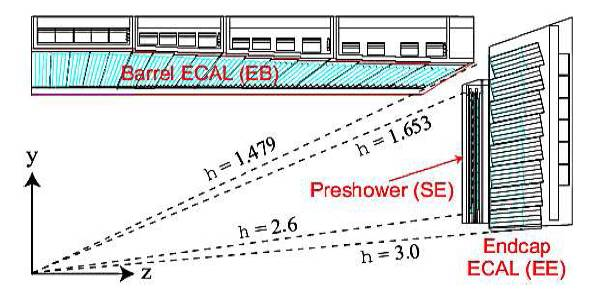
\includegraphics[width=3.8in, height= 3.0in]{pic/ecal} \\
    \caption{Longitudinal view of electromagnetic calorimeter. }
    \end{center}
    \end{figure}

%%% ----------------------------------------------------------------------
\subsection{Hadron Calorimeter-HCAL}
The Electromagnetic calorimeter is surrounded by Hadron
Calorimeter HCAL. The HCAL measure the energy of hadrons and
their products. HCAL is located at a distance of 1.77 m for the
interaction point. HCAL can be divided into four parts: barrel
(HB), end cap (EB), outer barred (HO) and Hadron forward
(HF).The barrel part covers the $\eta < 1.3$, Hadron End cap
covers the range from $1.3 <\eta < 3.0$. The Hadron End cap
receives high counting rates as compared to the barrel part.
For eta less than 1.3 Hadron Outer barrel (HO) is used to cover
this $\eta$ ranges. The forward calorimeter (HF) covers the
$\eta$ region up to 5.0. Here, the environment is very hostile
due to high radiation and energy deposition. Hence, quartz
fibers were chosen as calorimeter material. Particle showers
exceeding the Cerenkov threshold of $E > 190 KeV$ will be
detected. The segmentation in $\eta\times\phi$ is $0.175\times
0.175$ mm$^{2}$.

\subsection{Muon System}

The Muon system\index{muon system} of the CMS carries an immense importance. In
this outer most region of the detector only muon and neutrinos
can manage to pass through it without depositing their large
fraction of energy. The Muon system is developed to provide a
fast identification and efficient reconstruction. Three
different types of the gaseous detector are used in the muon
system which are RPC's, CSC and DT. In the barrel region four
layers of muon chambers are located along with Drift tubs. In
the end cap region $0.9 < \eta < 2.4$ Cathode strips are used
along with the RPC. The complete track of muon is obtained
after combining the information from the silicon tracker.  The
DT and CSC detectors are used to obtain a precise position
measurement, while the RPC's are, due to their very fast
response and time resolution of the order of 1 ns, dedicated
for timing information and the trigger
purpose\cite{muon1997,Cosmic}.
%\def\baselinestretch{1.66}
    \begin{figure}[h]
    \begin{center}
    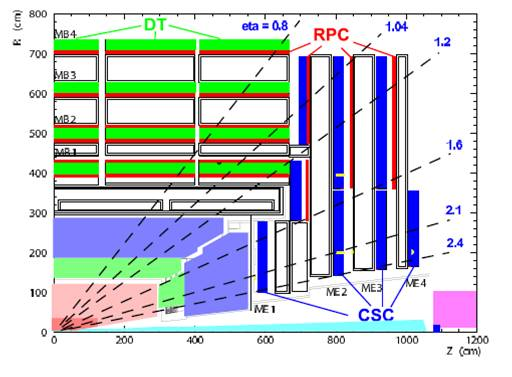
\includegraphics[width=3.5in]{pic/rpclayout} \\
    \caption{A section of detector where RPC are installed.}
    \end{center}
    \end{figure}
\smallskip
\subsection{The Trigger}
At the LHC, with a center-of-energy of 14 TeV and the
luminosity of $10^{34}$ cm$^{-2}$s$^{-1}$, the event rate is
about $10^{9}$ Hz and each event needs a typical space (event
size) of 1 MB. Therefore, the data stream coming from the
detector is around 1.2 TeraByte/s. It is therefore impossible
for the detector electronic system to record all events with
such a high frequency. The trigger system is used to select the
useful and interesting events and reduce the event rate to a
range manageable by the data acquisition system. The CMS
trigger system will reduce the event rate down to 100 Hz. This
reduction level is done through three levels of triggering. The
Level-1 (L1) reduces the rate to 100 kHz in the high luminosity
regime and 50 kHz for the low luminosity
phase~\cite{{hlt},{hlt1}}. The L1 decision to pass the event to
the next level of trigger must be taken in 3.2 $\mu$s. The L1
trigger uses only a coarse granularity information from
calorimeters and muon system because the decision must be taken
in a time which is very short to read all the data from the
whole detector. The High Level Trigger (HLT), which consists of
Level 2 and Level 3, is the second step of the trigger chain.
It has been designed to reduce the L1 output rate of 100 kHz to
the output rate of 100 Hz. The HLT code performs the
reconstruction and selection of physics objects using the full
event data with the granularity and matching information from
different sub-detectors. These objects are electrons, photons,
muons, missing energy, hadronic jets. The selection or
rejection of such objects allows to achieve the output rate of
100 Hz for events in the permanent storage medium.

\smallskip
\subsection{General Structure of the CMS trigger and DAQ}

The CMS trigger and data acquisition system (TriDAS) is designed to inspect the detector information at the full crossing frequency and to select events at a a maximum rate of O({$10 ^{2}$}Hz) for achieving and later off-line analysis. The CMSDAQ has to read out all front end electronic, to assemble the data from each bunch crossing into a single stand alone data structure, to provide these data to the processing element that execute the High Level Trigger (HLT).

The DAQ system provides the first place where the entire information from the physics collision can be inspected. It is also the place where the complete picture of the detector response to the collision can be monitored, thus providing early feedback to physicists running the experiment. 
    \begin{figure}[h]
    \begin{center}
    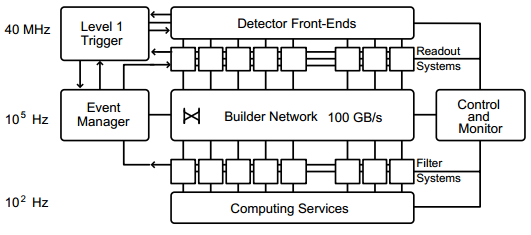
\includegraphics[width=3.5in]{pic/CERN_CMS_DAQ} \\
    \caption{Architecture of the CMS DAQ system}
    \end{center}
    \end{figure}
The DAQ is therefore the system that implement the two crucial function that exentually determine the reach of the physics program:\\
\smallskip
{\bf 1: Event selection.}\\
{\bf 2: Control and monitoring of the detector elements.}

The architecture of the CMS DAQ is shown in Fig 1.5 it consists of the following elements.\\
\smallskip 
1. {\bf Detectors front-ends:} The modules that store the data from the detectors front-end electronics upon the reception of a Level-1 trigger accept signal. the front end electronics are the responsible of the corresponding subdetectors. \\
2. {\bf Readout System:} The modules that read the data from the detectors front end electronics system. The data stored, untill they are sent to the processor, which will analyse the enent.\\
3.{\bf Builder network:} The collection of network that provides the interconnections b/w the readout and the filter system.\\
4.{\bf Filter system:} The processors, which are provided by the readout. They execute the HLT algorithum to select the events to be kept for off-line processing.\\
5.{\bf Event Manager:} The entity responsible for controlling the flow of data (events) in the DAQ system.\\
6. {\bf Computing services:} All the processor and networks that receive filtered events as well as a small fraction of rejected events from the filter farm.\\
7.{\bf Controls:} All the entities responsible for thr user interface and the configuration and monitoring of the DAQ.



%%% ----------------------------------------------------------------------


%% ------------------------------------------------------------------------
% -*-TeX-*- -*-Hard-*- Smart Wrapping
% ------------------------------------------------------------------------
% Thesis Acknowledgements ------------------------------------------------

\prefacesection{Acknowledgements}
\def\baselinestretch{0.5}
\setlinespacing{1.25}

I would like to thank Prof.Dr.Shahid A Khan my supervisor,
and Prof.Dr.Gilles Landeckar my Co-Supervisor for
many suggestions and constant support during this
research. He shared his knowledge and provided many useful
references and friendly encouragements. I am thankful to my colleagues
their positive criticism, continuous support and courage
through the early stages of chaos and confusion.\\

\indent\smallskip I am grateful to the Director Genral (NCP) Prof. Dr. Hafeez Hoorani, for allowing me to do research in National Center for Physics and Provide me fund to reaserch at European Council for Nuclear Research (CERN) to complete major part of this thesis.\\


\noindent
\begin{flushright}
Waqar Ahmed\\
\end{flushright}

% ----------------------------------------------------------------------


%% ------------------------------------------------------------------------
% -*-TeX-*- -*-Hard-*- Smart Wrapping
% ------------------------------------------------------------------------

\def\baselinestretch{1}

%\pagestyle{headings}

\chapter{Triple GEM detectors}

%\def\baselinestretch{1.5}


%%% ----------------------------------------------------------------------

\smallskip

%%% ----------------------------------------------------------------------
\goodbreak
\section{Small Prototype}







%%%----------------------------------------------------------------------------------------
\goodbreak
\section{Test Performed with the Small Prototypes}






%%%%--------------------------------------------------------------------------------------

\goodbreak
\textbf {X-ray generator used in the lab for gain calibration and uniformity measurements.}





%----------------------------------------------------------------------------------------

\smallskip
\textbf {Beam Test Setup}






%----------------------------------------------------------------------------------------

\smallskip

\goodbreak
\section{Full-Size Triple GEM detectors}






%%%--------------------------------------------------------------------

\smallskip
\section {The GE1/1-VI detector}






%---------------------------------------------------------------------------------------
\smallskip
\subsection{Mechanics}





%-----------------------------------------------------------------------------------
\smallskip
\subsection{GE1/1-VI Drift electrode and HV test}






%-----------------------------------------------------------------------------------

\smallskip
\subsection{GE1/1-VI GEM Foils}





%-----------------------------------------------------------------------------------
\smallskip
\subsection{HV Supply}






%-----------------------------------------------------------------------------------

\smallskip
\subsection{HV test of the GE1/1-VI GEM Foils}






%-----------------------------------------------------------------------------------

\smallskip
\subsection{GEM Electronics Board and Electronics}






%-----------------------------------------------------------------------------------
\smallskip
\subsection{Cooling}








%-----------------------------------------------------------------------------------
\smallskip
\subsection{HV Divider and Power Supply}






%-----------------------------------------------------------------------------------

\smallskip
\subsection{Assembly}






%-----------------------------------------------------------------------------------

\smallskip
\section{X-Ray radition test in the Lab}






%-----------------------------------------------------------------------------------
\smallskip
\subsection{Result from the test Beam }






%-----------------------------------------------------------------------------------
\smallskip
\section{conclusion}






%-----------------------------------------------------------------------------------



%% ------------------------------------------------------------------------
% -*-TeX-*- -*-Hard-*- Smart Wrapping
% ------------------------------------------------------------------------
\def\baselinestretch{1}
%\pagestyle{headings}

\chapter{Detector Control System}

%\def\baselinestretch{1.5}


%%% ----------------------------------------------------------------------

\smallskip

%%% ----------------------------------------------------------------------
\goodbreak
\section{Data Acquisition System in CMS . . . . . .}


%%%----------------------------------------------------------------------------------------
\goodbreak
\section{The Detector Control System}


%------------------------------------------------------------------------------------

\smallskip
\subsection{General Requirements}

%-----------------------------------------------------------------------------------
\smallskip
\subsection{DCS Architecture}

%-----------------------------------------------------------------------------------

\smallskip
\section{DCS Software tools}

%-----------------------------------------------------------------------------------
\smallskip
\subsection{Wincc OA}

%-----------------------------------------------------------------------------------

\smallskip
\subsection{JCOP Framework}

%-----------------------------------------------------------------------------------

\smallskip
\section{The GEM DCS : Hardware system}

%-----------------------------------------------------------------------------------
\smallskip
\subsection{Power System}


%-----------------------------------------------------------------------------------
\smallskip
\subsection{High Voltage and Low Voltage System}
%-----------------------------------------------------------------------------------

\smallskip
\subsection{Temperture System}

%-----------------------------------------------------------------------------------

\smallskip
\subsection{Cooling System}

%-----------------------------------------------------------------------------------
\smallskip
\subsection{Enviroment System}

%-----------------------------------------------------------------------------------


\smallskip
\section{Design and Development of the GEM DCS}

%-----------------------------------------------------------------------------------

\smallskip
\subsection{Finate state Machine}

%-----------------------------------------------------------------------------------

\smallskip
\subsection{Alrm Handling}

%-----------------------------------------------------------------------------------

\smallskip
\subsection{Configuration Datbase}

%-----------------------------------------------------------------------------------

\smallskip
\subsection{The graphical User Interface}

%-----------------------------------------------------------------------------------

\smallskip
\subsection{Intergration in the Central CMS GEM DCS}

%-----------------------------------------------------------------------------------

\smallskip
\section{Conclusion}

%-----------------------------------------------------------------------------------




%\include{concl}


%\appendix
%\input{AppendixA.tex}
% ------------------------------------------------------------------------
\setlinespacing{1.1}
\bibliographystyle{unsrt}
\bibliography{XBib}
% =================================================================
%\printindex
\end{document}
% ------------------------------------------------------------------------


